\documentclass[10pt,letterpaper]{article}
\usepackage[margin=0.8in]{geometry}
\usepackage[T1]{fontenc}
\usepackage[utf8]{inputenc}
\usepackage{lmodern,xcolor,tabularx,booktabs,array,enumitem,hyperref,fancyhdr,lastpage,titlesec,amsmath,microtype,needspace,ragged2e,graphicx}
\definecolor{navy}{HTML}{19334C}
\definecolor{teal}{HTML}{236B82}
\definecolor{muted}{HTML}{52616B}
\hypersetup{colorlinks=true,linkcolor=teal,urlcolor=teal,pdftitle={Group Number 11: Human or AI?}}
\titleformat{\section}{\Large\bfseries\color{navy}}{\thesection.}{0.6em}{}
\titlespacing*{\section}{0pt}{14pt}{7pt}
\setlength{\parindent}{0pt}\setlength{\parskip}{4pt}\setlength{\headheight}{15pt}
\renewcommand{\arraystretch}{1.12}
\newcolumntype{Y}{>{\RaggedRight\arraybackslash}X}
\newcommand{\q}[2]{\needspace{4\baselineskip}\par\addvspace{7pt}\textbf{#1}\quad\textit{#2}\par\nobreak}
\pagestyle{fancy}\fancyhf{}
\fancyhead[L]{\small\color{muted}Cornell Tech | Applied Machine Learning}
\fancyhead[R]{\small\color{muted}Group Number 11}
\fancyfoot[C]{\small\color{muted}Page \thepage\ of \pageref{LastPage}}
\begin{document}
\thispagestyle{empty}
{\color{teal}\bfseries CORNELL TECH | APPLIED MACHINE LEARNING}\par
\vspace{0.18in}
{\Huge\bfseries\color{navy}Human or AI?}\par
\vspace{0.07in}
{\LARGE\color{navy}Style-aware text classification}\par
\vspace{0.16in}
\textbf{Kaggle competition report | Group Number 11}\par

November 11, 2026\par\vspace{0.1in}
\begin{tabularx}{\linewidth}{@{}Yr@{}}
\toprule
Team member & NetID \\ \midrule
Ansh Raj Bhargava & \texttt{ab3396} \\
Yilin Gao & \texttt{yg695} \\
Yingzi Gu & \texttt{yg667} \\
\bottomrule
\end{tabularx}

\textbf{GitHub PR:} \url{https://github.com/sekhari/human-or-ai-submissions/pull/13}\par
\textbf{Submission branch:} \texttt{submission/group-number-11}. Development branch: \texttt{Group11retry}.
\section*{Team information and model summary}
\q{Q0.1}{Team and contributions.}Yilin Gao (yg695) led model development and comparison (Q1): data inspection, the shared split, representations, baseline comparisons and tuning. Ansh Raj Bhargava (ab3396) led the unlabeled-data and improvement experiments (Q3 and Q5). Yingzi Gu (yg667) led learning curves, subgroup evaluation and error analysis (Q2 and Q4). All three members also trained models and explored stronger configurations. These roles were supplied by the team; the implementation and experiment execution in this rebuilt branch were assisted by Codex. Individual AI-use disclosures appear in Q6.3.
\q{Q0.2}{Final approach.}
The final score is $\sigma(0.75\,\mathrm{logit}(p_N)+0.25\,\mathrm{logit}(p_M))$, where $p_N=\sigma(0.9\,\mathrm{logit}(p_L)+0.1\,\mathrm{logit}(p_R))$ and probabilities are clipped before logit conversion.
The parent $p_L$ blends a GPT-2/statistics LightGBM (75\%) with the original word/character/style ensemble (25\%).
The neural branch $p_R$ fine-tunes the upper four RoBERTa blocks on 8,000 training rows, with random token crops and first/last-window inference.
The detector $p_M$ combines frozen small/medium GPT-2 statistics and local style features with label-free within-format score alignment.
A fixed 2,000-row holdout selects the configurations; tree components are then refitted on all 10,000 labels while RoBERTa retains its held-out checkpoint, and all models run locally without external authorship labels or hosted prediction APIs.
\q{Q0.3}{Recorded scores.}
\par\noindent
\begin{tabularx}{\linewidth}{@{}Yr@{}}
\toprule
Metric & AUROC \\ \midrule
Final fixed validation & 0.999822 \\
Initial public (earlier team model) & 0.92433 \\
First rebuild public & 0.96962 \\
Final optimized public (team-reported) & 0.98921 \\
Kaggle private & Not revealed \\
\bottomrule
\end{tabularx}

\par
\textbf{Interpretation.} The public result comes from the team\textquotesingle s Kaggle submission report. It is 0.010612 below validation. Repeated holdout selection and hidden-domain differences limit generalization claims; private performance remains unknown.
\newpage
\section{Model comparison and selection}
\q{Q1.1}{Preprocessing and representations.}
We decode literal backslash-n and backslash-t sequences into actual whitespace without discarding case, punctuation or paragraph boundaries.
Word TF-IDF uses scikit-learn's default word token pattern, 1--2 grams, minimum document frequency 2, maximum document frequency 0.995, Unicode accent stripping, sublinear term frequency, L2 normalization and at most 180,000 features.
Character TF-IDF uses 2--5 grams, minimum document frequency 3, sublinear term frequency, L2 normalization and the same feature cap.
Our custom preprocessor preserves case, including for word features.
Style features measure lexical diversity, hapax frequency, word/sentence lengths, punctuation, paragraph structure, function-word rates and several simple regex patterns.
These represent complementary lexical and structural evidence.
Each vocabulary and IDF transform is fitted on training texts only; row-local style extraction learns no corpus statistics.
\q{Q1.2}{Model comparison on the same validation set.}
\begin{tabularx}{\linewidth}{@{}Yrrr@{}}
\toprule
Model / features & Train AUC & Val. AUC & Seconds \\ \midrule
Word LR, $C=4$ & 1.000000 & 0.949536 & 2.51 \\
Word linear SVM, $C=1$ & 1.000000 & 0.952006 & 2.45 \\
Character LR, $C=16$ & 1.000000 & 0.977193 & 16.96 \\
Word NB-weighted LR, $C=4$ & 0.972718 & 0.938555 & 2.47 \\
Style LightGBM, 31 leaves / 700 trees & 1.000000 & 0.997234 & 5.75 \\
Initial three-component blend & 1.000000 & 0.997975 & Shared fits \\
\bottomrule
\end{tabularx}

\small Times are local CPU feature-construction plus classifier-fit wall time, excluding scoring and checkpoint I/O; shared feature construction is attributed to each setting. They are approximate, not a hardware benchmark.\normalsize
\q{Q1.3}{Hyperparameters and selection protocol.}
\begin{tabularx}{\linewidth}{@{}YYl@{}}
\toprule
Approach & Candidates & Selected \\ \midrule
Word LR / SVM & $C\in\{0.1,1,4,16\}$ & SVM, $C=1$ \\
Character LR / SVM & $C\in\{0.1,1,4,16\}$ & LR, $C=16$ \\
NB-weighted LR (both representations) & $C\in\{0.1,1,4\}$ & Not retained \\
Style LightGBM & Leaves $\{7,15,31\}$; trees $\{300,700\}$ & 31 / 700 \\
\bottomrule
\end{tabularx}

Seed 20261023 fixes a stratified 8,000/2,000 split. We compare 28 base settings and select the highest validation AUC within each representation.
LightGBM uses learning rate 0.03, minimum child size 40, feature fraction 0.85 and L2 regularization 5.
We evaluate 15 blend-grid entries: style weight $s\in\{0,.25,.5,.75,1\}$, with remaining weight divided between word and character components using $c\in\{0,.5,1\}$. Thus weights are $((1-s)(1-c),(1-s)c,s)$; pure-style endpoints repeat.
For this initial grid, settings were selected without Kaggle feedback or test labels; later public-feedback decisions are recorded separately. Reusing one validation set can still produce selection optimism.
\q{Q1.4}{Final model choice and later changes.}
The first rebuild achieved 0.96962 public AUROC. A format-robust candidate dropped to 0.95899, so it was rejected.
Frozen language features then raised public AUC to 0.98665; a small RoBERTa logit contribution raised it to 0.98861.
The final selected submission scores 0.999822 validation / 0.98921 public AUROC.
These later changes add complementary representations while retaining a large contribution from the previously scored detector.
The neural-only validation AUC was 0.979583, so sophistication alone did not justify replacing the stronger parent.
Small blend gains on the reused validation partition are not statistically decisive; public feedback is recorded separately and private performance is unknown.
The appendix records the pretrained sources, training schedules, blend search and compute cost. Scores optimize ranking, not calibrated authorship certainty.
\newpage
\section{Effect of training data size}
\q{Q2.1}{Controlled learning curve.}
We fix word logistic regression at $C=4$ and use stratified samples from the same 8,000-row training partition with seed 20261023. Each size gets a freshly fitted vocabulary and IDF, preventing smaller training sets from borrowing the full corpus representation. The 2,000 validation examples are unchanged. The smaller subsets are sampled separately; nesting is not required for this comparison.

\begin{tabularx}{\linewidth}{@{}lrrr@{}}
\toprule
Training rows & Training AUROC & Validation AUROC & Seconds \\ \midrule
500 & 1.000000 & 0.853259 & 0.28 \\
1000 & 1.000000 & 0.901718 & 0.41 \\
2000 & 1.000000 & 0.922063 & 0.64 \\
5000 & 1.000000 & 0.939543 & 1.40 \\
8000 & 1.000000 & 0.949536 & 2.22 \\
\bottomrule
\end{tabularx}

\q{Q2.2}{Learning-curve figure.}
\begin{center}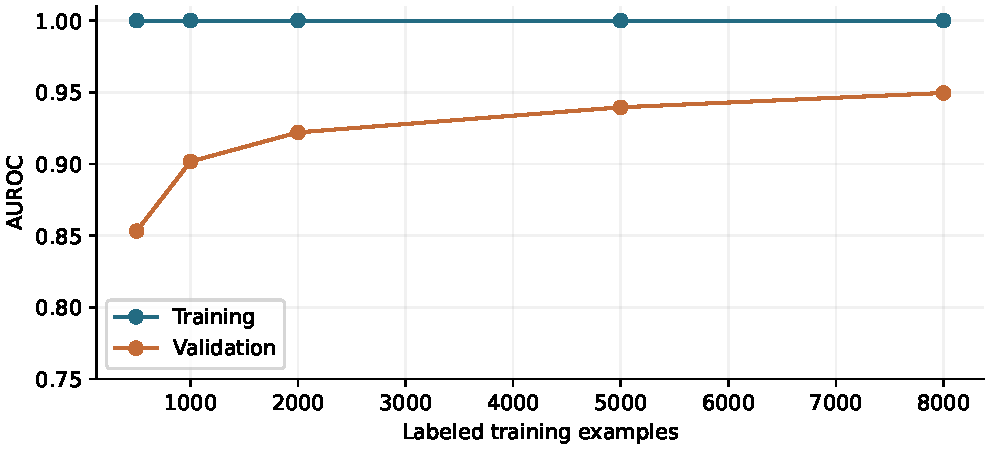
\includegraphics[width=.96\linewidth]{learning_curve.pdf}\end{center}
\q{Q2.3}{Interpretation.}
Training AUC is 1.0 at every size, whereas validation AUC increases from 0.853259 at 500 examples to 0.949536 at 8,000.
This is an overfitting pattern: a high-dimensional linear classifier separates its own examples even when the learned vocabulary and weights do not generalize as well.
The increase from 5,000 to 8,000 examples is about 0.0100, so additional labeled data remains useful for this configuration.
The curve does not show substantial training underfitting and does not establish that this model has saturated.
Only one sample per size is measured; the curve has sampling variability, and no asymptotic rate is inferred.
It is a learning curve for word LR, not evidence that the final style-heavy blend would improve by the same amount.
\newpage
\section{Learning from unlabeled data}
\q{Q3.1}{Method and leakage prevention.}
We test unsupervised representation learning using the additional 3,000 unlabeled texts.
The supervised baseline fits word vocabulary and IDF only on the 8,000 training texts.
The alternate representation fits vocabulary and IDF on these same texts plus all 3,000 unlabeled texts.
Both classifiers use logistic regression with $C=4$ and train on exactly the same 8,000 true labels.
Neither validation texts nor validation labels enter either representation fit, and test texts are excluded.
This experiment does not create pseudo-labels or assume unlabeled authorship.
The fixed holdout isolates the effect of changing corpus statistics, although it cannot establish whether the same change would help hidden test domains.
\q{Q3.2}{Measured comparison.}
\begin{tabularx}{\linewidth}{@{}Yr@{}}
\toprule
Method & Validation AUROC \\ \midrule
Supervised word LR only & 0.949536 \\
Training + unlabeled vocabulary/IDF & 0.949414 \\
\bottomrule
\end{tabularx}

\q{Q3.3}{Did unlabeled data help?}
No improvement was observed: validation AUC changes by
-0.000122
.
This difference is tiny and should be interpreted as essentially neutral rather than strong evidence of harm.
Additional documents change vocabulary coverage and IDF weights but supply no new class information.
They may add domain vocabulary that is not useful for authorship discrimination; this is a hypothesis, not a measured causal explanation.
Pseudo-label noise cannot explain this result because no pseudo-labels were used.
The baseline component therefore retains its supervised-only word representation fit.
A future self-training experiment would need a fixed confidence rule, comparison on the same holdout, and explicit checks for confirmation bias rather than an assumption that more unlabeled data always helps.
\vspace{.15in}
\textbf{Data accounting.} The starter file is a subset of the supplied labeled set and is never appended as additional training data. The 3,000 test texts are used only for inference. No hidden labels are recovered from the dataset's external source or from external model services.
\newpage
\section{Generalization and error analysis}
\q{Q4.1}{Final training--validation gap and uncertainty.}
The final selected model has training AUC 1.000000 and validation AUC 0.999822. These scores use the controlled 8,000/2,000 fit before full-data refitting. A 1,000-replicate stratified bootstrap gives [0.999629, 0.999948], conditional on the selected fitted model; it excludes selection and distribution-shift uncertainty.
No exact texts cross the split. Two validation passages have nearest-training word-TF-IDF cosine similarity at least 0.90; removing them yields AUC 0.999822. This is not a complete shared-source audit.
The public AUC is lower than random-split AUC. That observed gap, and the failed robust candidate, caution against treating a near-perfect holdout as a universal authorship detector.
The training AUC is exactly rank-certified from bounded, clipped-logit ensemble scores; this avoids unnecessary full neural inference on the training partition. The certificate and bounds are saved with the analysis.
\q{Q4.2}{Final observable text-length subgroups.}
We count whitespace-delimited words after decoding escaped newlines and keep the original bins, independent of labels and model predictions.

\par\noindent
\begin{tabularx}{\linewidth}{@{}Yrrr@{}}
\toprule
Words & Count & Human / AI & AUROC \\ \midrule
0 <= words < 150 & 380 & 146 / 234 & 0.999854 \\
150 <= words < 250 & 1049 & 605 / 444 & 0.999814 \\
words >= 250 & 571 & 249 / 322 & 0.999888 \\
\bottomrule
\end{tabularx}

\par
All three bins have AUC near 1.0. Unequal group sizes and tiny differences do not establish a reliable subgroup advantage. These length groups do not test new generators or domains; the appendix adds unsupervised topic/style-cluster checks, which are also only proxies.
\begin{center}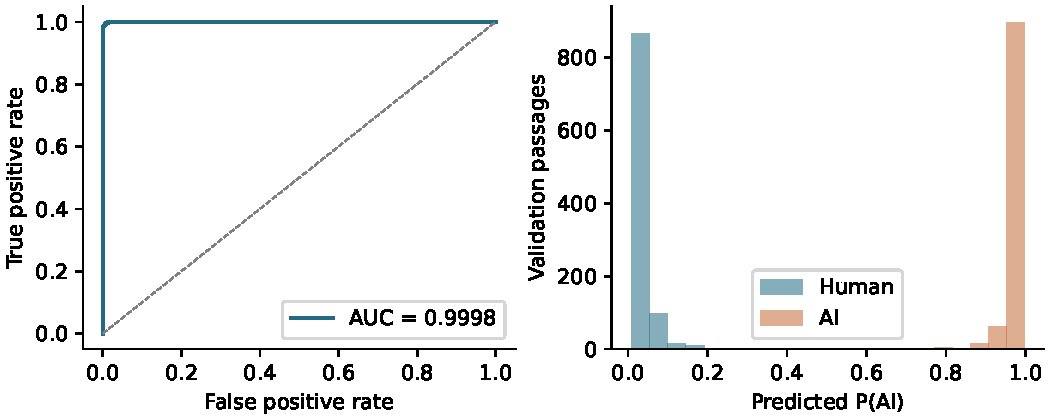
\includegraphics[width=\linewidth]{diagnostics_optimized.pdf}\end{center}
\q{Q4.3}{Final-model error review.}The final confusion matrix is TN=996, FP=4, FN=12, TP=988, with accuracy 0.9920. These counts use threshold 0.5. For the required five-FP/five-FN case review we use threshold 0.40, yielding 6 FP and 10 FN. This review threshold is stated explicitly and does not change AUROC or the continuous Kaggle predictions. The next page shows the five highest-scoring human false positives and five lowest-scoring AI false negatives under that review threshold.
\newpage
{\Large\bfseries\color{navy}Generalization: concrete errors}\par
All error labels below use the declared review threshold 0.40. The descriptions come from reviewing the supplied validation passages. Proposed explanations are hypotheses; we did not intervene on each passage to establish causation.


\par\noindent

\par\noindent
\begin{tabularx}{\linewidth}{@{}rrrY@{}}
\toprule
ID & Error & Final P(AI) & Observed content / hypothesis \\ \midrule
2696 & FP & 0.9277 & Human-labeled forum text repeats long phrases extensively; repetition is a plausible misleading generation cue. \\
7384 & FP & 0.6066 & Very short film review with broad judgments; limited text makes style estimates uncertain. \\
6138 & FP & 0.5737 & Formal historical description with many named entities overlaps the style of generated summaries. \\
9585 & FP & 0.5156 & Fluent encyclopedia biography with repeated names, dates and media titles resembles generated reference prose. \\
921 & FP & 0.4244 & Formal definitional exposition repeats abstract concepts and resembles generated explanatory prose. \\
7049 & FN & 0.0995 & Recipe quantities, bullets and personal restaurant commentary resemble human recipe/blog material. \\
3457 & FN & 0.1625 & Quoted, line-wrapped academic abstract looks like source material; formatting and vocabulary may mask authorship cues. \\
9298 & FN & 0.2005 & Biography-like prose with dates, names and irregular spacing resembles human reference writing. \\
3061 & FN & 0.2301 & Quoted parenting discussion uses informal, personal language that resembles human forum text. \\
1689 & FN & 0.2664 & Dense mathematical notation and code fences are poorly represented by English predictability statistics. \\
\bottomrule
\end{tabularx}

\par


\par


\q{Q4.4}{Recurring errors and changes after blending.}
The reviewed cases include repetitive human wording, reference/review prose and structured exposition, alongside AI content with recipe, academic, reference and conversational framing.
These genres overlap across labels: predictability, conversational irregularity and technical notation do not uniquely identify authorship.
The final model has 16 total errors at the common threshold 0.5, compared with 18 for the language parent and 31 for the first rebuild. The ten detailed examples use the separately declared review threshold.
The mechanism descriptions are hypotheses based on observed text, not causal interventions or recovered generator identities.
More targeted training-only symbolic-text augmentation could be tested, but was not assumed to work.
The small public subset and repeated model selection still limit conclusions about unseen generators and private performance.
\newpage
\section{Open-ended improvements and insights}
\q{Q5.1}{Hypothesis.}
Lexical models and style features should make different errors, so their blend may improve ranking over either representation alone.
The fixed-holdout results support this as a useful experiment: the character model is substantially weaker than style boosting but can still contribute complementary information.
After the blend experiment, feature-gain inspection showed paragraph-format dependence. We therefore also tested whether whitespace augmentation could preserve native-text AUC while improving robustness to a formatting shift.
This second question matters because random splits retain acquisition and formatting regularities that may not survive different preprocessing or adversarial edits.
\q{Q5.2}{Exact changes and controlled comparison.}
For the blend improvement, we keep the labeled split and trained components fixed and change only the mixture weights, using the finite grid described in Q1.3.
For the augmentation follow-up, each training passage contributes its original and whitespace-collapsed version with the same supplied label.
The 8,000 source training passages become 16,000 transformed training rows, not additional independent labeled examples.
We compare 15- and 31-leaf style models with 700 trees and style weights 0.75 or 1.0; lexical components stay fixed.
Before executing this follow-up, we specified an acceptance rule: native AUC must be within 0.0005 of the original blend and collapsed-text AUC must be at least 0.98. Eligible candidates would be ranked by native AUC.
\q{Q5.3}{Measured results.}
\begin{tabularx}{\linewidth}{@{}Yrr@{}}
\toprule
Configuration & Native AUC & Collapsed AUC \\ \midrule
Character LR alone & 0.977193 & Not isolated \\
Style boosting alone & 0.997234 & Not isolated \\
Initial three-component blend & 0.997975 & 0.877512 \\
Augmented 31-leaf style + lexical blend & 0.997503 & 0.978602 \\
\bottomrule
\end{tabularx}

The selected blend reuses the component fits from Q1.2; prediction adds three component passes.
The 31-leaf augmented candidate takes
6.57
 seconds for feature construction and fitting with cached original features; this excludes the already fitted lexical components and is not a full-pipeline speed comparison.
Removing size and sentence/paragraph-count features from the original style model yields AUC
0.996225
 (baseline 0.997234). This partial ablation still retains newline-character frequency, so it does not establish formatting independence.
\q{Q5.4}{What we learned and limitations.}
Blending gives a small native-text ranking improvement, but it does not solve formatting dependence.
Whitespace augmentation raises collapsed-text AUC from 0.877512 to 0.978602 for the strongest native-text augmented candidate, while reducing native AUC from 0.997975 to 0.997503.
No candidate passes the prespecified 0.98 collapsed-text requirement, so augmentation alone was rejected; the later language-feature model is evaluated in the appendix.
ASCII punctuation normalization retains AUC 0.997797, and bracket-reference removal retains 0.997425; whitespace is the clearly larger measured vulnerability.
The three frozen-setting secondary random splits score
0.998941, 0.997419, 0.998878
. They support random-split stability but overlap the selection pool and do not constitute external validation.
These results support the narrow claim that the model ranks supplied unmodified validation passages well.
They do not establish robustness to hidden adversarial transformations or a specific Kaggle score.
A next experiment would canonicalize formatting throughout training and inference and compare its worst-transformation AUC under a separately reserved evaluation protocol.
\newpage
\section{Code, reproducibility and AI assistance}
\q{Q6.1}{PR, environment and entrypoints.}
\textbf{PR URL:}
\url{https://github.com/sekhari/human-or-ai-submissions/pull/13}

\textbf{Location:} \texttt{submissions/group-number-11/}.\par
Initial baseline versions are recorded in \texttt{environment.txt} and \texttt{requirements.txt}.
For the final model, activate the project virtual environment and install \texttt{requirements-optimization.txt}; the exact added package versions are pinned there.
The tested setup uses Python 3.14.2 on macOS arm64 with Apple MPS; CPU fallback is available but slower.
The split/tree seed is 20261023 and the neural seed is 20261111; supplementary split seeds are 20261024--20261026.
The reproduction command trains/evaluates the components; the prediction command below regenerates the CSV from their cached inference outputs without reselecting weights or reading validation labels.
\begin{quote}\footnotesize\begin{verbatim}
pip install -r submissions/group-number-11/requirements-optimization.txt
DATA_DIR=cornell-tech-cs-5785-combined-2026-ai-vs-human-text
bash submissions/group-number-11/reproduce_final.sh "$DATA_DIR"
python submissions/group-number-11/predict_final.py \
  --data "$DATA_DIR" \
  --out submissions/group-number-11/output/submission.csv
\end{verbatim}\end{quote}
The reproduction script recreates the components; \texttt{predict\_final.py} writes the frozen blend from cached inference outputs. Data, model weights and caches are excluded from Git.
\q{Q6.2}{Development history and lessons.}\begin{itemize}[leftmargin=1.5em,itemsep=3pt]
\item \href{https://github.com/hisylvia66/human-or-ai-submissions/commit/e31a805}{e31a805}: Build fixed-holdout text and stylometric training pipeline
\item \href{https://github.com/hisylvia66/human-or-ai-submissions/commit/09c05b0}{09c05b0}: Test format-robust classifiers and document negative public result
\item \href{https://github.com/hisylvia66/human-or-ai-submissions/commit/f8c557e}{f8c557e}: Add frozen GPT-2 detector reaching 0.98665 public AUROC
\end{itemize}The initial pipeline established the shared split and baseline comparisons. The format-robust follow-up showed that synthetic stress improvement did not transfer to public performance. The language-feature change then improved both the fixed validation score and the user-reported public score. These are actual development checkpoints; the experiments and their negative results are retained for review.
\newpage
\section*{AI assistance and individual contributions}
\q{Q6.3}{AI assistance and verification.}
OpenAI Codex assisted Yingzi Gu with pipeline design, code, debugging, experiment execution, analysis and report drafting.
Experiments were run locally on the supplied data; offline scores come from their logs, while the public score was supplied by the team.
Automated checks verify the fixed split, validation labels/AUC, data hashes, output IDs/order and finite probability bounds.
No hosted LLM API labeled or predicted passages. Optimization used generic GPT-2 weights locally and fine-tuned upper RoBERTa blocks using only supplied labels; additional neural experiments are recorded in the optimization logs. No external authorship labels were used.
Team-reported roles appear in Q0.1; the team must review the submitted code and interpretations.
The individual disclosures below also cover earlier experiments retained in the merged team history.

OpenAI ChatGPT assisted Yilin Gao with baseline implementation, model comparison and hyperparameter-tuning code, result interpretation, GitHub/reproducibility setup, and drafting parts of Q1. Yilin reviewed the code, experimental outputs, and report content before committing or incorporating them.

Ansh used Claude (Anthropic) for help with the experiment code for the unlabeled-data and robustness studies (Q3 and Q5), including the self-training and pseudo-labeling pipeline, the normalization and augmentation experiments, data loading and the Kaggle notebook setup, GitHub workflow and reproducibility setup, result interpretation, and drafting parts of Q3 and Q5. Ansh ran the experiments on Kaggle and reviewed the code, experimental outputs and report content before committing or incorporating them.

\vspace{.1in}
\textbf{Sources.} The supplied \emph{Kaggle Competition Template Report} PDF/LaTeX provides the protocol and Q0--Q6 requirements; the course README provides the repository layout. Offline results come from saved experiment logs; public results were supplied by the team. No external label source was consulted.
\vspace{.1in}
\textbf{Submission status.}
The team reported public AUROC 0.98921 for the optimized submission, following 0.96962 for the first rebuild and 0.92433 for the earlier model. Private results remain pending. See the title page for the course PR.

\textbf{Compute and limitations.} Language-feature extraction took minutes on the local Apple GPU and is cached for reuse; the language-parent classifier stage took about 23 seconds with cached features. This is not directly comparable to the initial CPU feature-plus-fit timings. The final tree fits use all 10,000 true labeled rows after selection, with paired style views counted as augmentation rather than new independent data. Generic pretrained language knowledge is the only added external model resource. Public feedback was used to reject the robust candidate and confirm the language candidate; no hidden individual labels were accessed. The repeated holdout search and small public subset remain sources of selection uncertainty.

\newpage
\section*{Appendix: post-submission optimization (Q1/Q5/Q6 continuation)}
\textbf{Measured sequence and selection.} The first format-robust candidate improved synthetic stress AUC but reduced public AUC, an informative negative result. The language-feature candidate was then selected using the original fixed holdout: retain at least 25\% baseline weight, require native AUC at least 0.9975, and maximize 0.75 times the no-blank-line subgroup AUC plus 0.25 times overall AUC. This focuses on passages without an easy paragraph cue. A finite grid compared baseline weights 0.25, 0.5 and 0.75, with plain or conditional-rank blending. Plain blending won for the language parent. The later medium detector uses label-free conditional-rank alignment within observed blank-line groups; no true labels enter inference.

\par\noindent
\begin{tabularx}{\linewidth}{@{}Yrr@{}}
\toprule
Configuration & Validation AUC & Public AUC \\ \midrule
First rebuild ensemble & 0.997975 & 0.96962 \\
Robust format candidate & 0.995598 & 0.95899 \\
GPT-2 statistics + baseline & 0.999785 & 0.98665 \\
RoBERTa logit hybrid & 0.999805 & 0.98861 \\
Medium-language hybrid & 0.999822 & 0.98921 \\
\bottomrule
\end{tabularx}

\par
\textbf{Representation and search.} The additional 279-dimensional representation includes the original 160 style features plus lexical-diversity, n-gram repetition, word/sentence distributions and character/paragraph statistics. We concatenate 26 frozen GPT-2 features: token negative-log-likelihood distribution statistics, head/tail-window statistics, rank-1/10/100 fractions and logit-margin statistics. Only the first 256 model tokens are used.
The generic model is \href{https://huggingface.co/openai-community/gpt2}{openai-community/gpt2}, revision \texttt{607a30d783dfa663caf39e06633721c8d4cfcd7e}; its pretrained weights are unchanged. No competition passage is sent to a hosted endpoint.
The new grid compares LightGBM leaves 7/15/31 and CatBoost depth 5 in native, collapsed and paired native/collapsed style views. Language features retain original text in those paired style views, so style-only stress scores are not reported as full-pipeline format robustness.

\textbf{Additional grouped evidence.} Twelve unsupervised lexical topic/style clusters define three group-held-out folds, without hidden source labels. Frozen style-only and style-plus-GPT-2 configurations use their separately selected 31- and 15-leaf settings. This is a pipeline comparison, not an isolated feature ablation:

\par\noindent
\begin{tabularx}{\linewidth}{@{}Yrr@{}}
\toprule
Fold & Style only & Style + GPT-2 \\ \midrule
1 & 0.994101 & 0.999002 \\
2 & 0.998777 & 0.998415 \\
3 & 0.990991 & 0.997209 \\
\bottomrule
\end{tabularx}

\par
The small regression on fold 2 cautions against universal improvement claims. These clusters are proxies, and their folds overlap the original selection pool; they are not independent external confirmation.

\textbf{Neural continuation.} The generic source is \href{https://huggingface.co/FacebookAI/roberta-base}{FacebookAI/roberta-base}.\par
Revision: \texttt{e2da8e2f811d1448a5b465c236feacd80ffbac7b}.\par
Embeddings and the lower eight encoder blocks are frozen; four upper blocks and a fresh classification head train on the 8,000 training examples. AdamW uses learning rates $2\cdot10^{-5}$ for the encoder and $10^{-4}$ for the head, weight decay 0.01, batch size 16 and seed 20261111.
Canonicalized texts receive random 192-token crops; inference averages first/last windows. A budgeted two-epoch attempt stopped at step 861; validation chose checkpoint 750. The tree parent is later refitted on 10,000 rows, while the neural branch retains its 8,000-row checkpoint.
Plain and logit blends at neural weights 0/.05/.1/.15/.25/.5 were compared; 0.1 logit blending won by validation AUC (0.999805 versus 0.999785). This tiny local difference is not conclusive evidence; the public result 0.98861 was supplied independently by the team.
\textbf{Second language model.} Frozen \href{https://huggingface.co/openai-community/gpt2-medium}{GPT-2-medium} uses canonical whitespace and a 128-token prefix, alongside the small model's 256-token features. Their statistics, differences and normalized ratios give 104 language dimensions, not a same-context theoretical perplexity ratio. A native-view 31-leaf LightGBM uses these plus the 279 style features. Its scores receive label-free within-format quantile alignment to the reference detector, then 75\% aligned scores are combined with 25\% reference scores to form $p_M$. The final grid compares plain/logit weights .25/.5/.75 for $p_M$, retaining at least 25\% of the scored neural hybrid. A 25\% logit contribution wins. The rank mapping uses only predicted scores and observed blank-line groups, never true test labels.


\end{document}
